% !TEX root = diss.tex

\chapter{The Relationship Between Arrhenius Pre-factors with Non-Covalent Binding}
\label{ch:arrhenius}

In the paper by DiLabio and Ingold\cite{DiLabio2005} investigating the formal HAT reaction of the iminoxyl/oxime self-exchange reaction, they compiled a table of parameters from the phenomenolical Arrhenius equation for a series of interesting reactions.\cite{Kreilick1966, Mader2004, Mahoney1970, DaRooge1967, Howard1973, Foti1994, Chenier1974, Chenier1975} These are self-exchange reactions of oxygen-centred $\pi$-radicals\footnotemark~and other thermoneutral (or nearly thermoneutral) reactions involving the destruction and formation of oxygen-centred $\pi$-radicals, reactions 3.1 and 3.2, respectively:

\footnotetext{\noindent $\pi$-radicals are those in which the singly-occupied molecular orbital (SOMO) is orthogonal to the plane of the molecular framework, i.e.\ of $\pi$-symmetry. Note that free alkoxyl radicals cannot be distinguished as either $\sigma$ or $\pi$-radicals, as the SOMO is free to rotate with respect to the rest of the molecular framework. Therefore, only the geometry of the radical-molecule complex can determine the symmetry of the SOMO.}

\begin{align}
  \ch{$\pi$-RO^. + ROH &-> ROH + $\pi$-RO^.} \hspace{2cm} \Delta H = 0 \\
  \ch{$\pi$-R}^\prime\ch{O^. + ROH &-> R}^\prime\ch{OH + $\pi$-RO^.} \hspace{2cm} \Delta H \approx 0
\end{align}

Although it is well known that reactions of this nature involve remarkably low activation energies ($E_a$),\cite{Lucarini1996,Mahoney1970a,Mahoney1975,Korcek1972} they also have unusually low Arrhenius pre-exponential factors ($A$), or as we shall refer to them, \emph{A-factors}, leading to slower than expected reactions; summarised in~\ref{tab:Arrhenius}.
adThe measured A-factors range fromm $10^{3.5}$--$10^{8.3}$ \Ms, while normally HAT reactions are typically $10^{8.5\pm0.5}$ \Ms.\cite{Benson1976} This is likely due to steric shielding around the oxygen atoms, resulting in a large entropic barrier.\cite{DiLabio2005} Additionally, it was noted that the degree of steric shielding on the oxygen atom appears to play an important role in the order of the A-factor; systems with greater bulk have lower A-factors while non-shielded systems have larger A-factors.

Steric-electronic effects play an important role in HAT, and have been studied extensively by our colleagues in Rome, as well as by others.\cite{Finn2004,Salamone2011,Pischel2001,Griller1981,Bietti2011, Salamone2012,Malatesta1982,Salamone2014} Although a C-H bond may be weaker than others on a given substrate, if it is not accessible due to steric constraints, abstraction will not occur at this site. Otherwise, additional steric bulk can lead to significant reductions in reactivity, through destabilisation of the TS complex. For example, in reactions of tertiary acetamides with \cumo,\cite{Salamone2014} where abstraction occurs mainly from C-H bonds $\alpha$ to the nitrogen atom, a two fold decrease in normalised rate constant is observed in going from $N,N$-dimethylacetamide to $N,N$-diisobutylacetamide ($k_H$ = $2.0 \times 10^5$ and $7.8 \times 10^4$ \Ms, respectively).

Upon first inspection, all of the reactions in~\ref{tab:Arrhenius} appear to be fairly similar in nature. That is, the bonds formed and broken in all cases are comparable and should not contribute significantly to reaction barrier in a Bell-Evans-Polanyi principle fashion. Hence, the large degree of variance in their rate constants ($k$) is somewhat surprising. For the closely related self-exchange reaction between phenol and phenoxyl,\cite{Mayer2002} a strong molecule-radical pre-reaction complex is formed, ca. 10 \kcalmol below the separated reactants. It is therefore expected that most, if not all, of the systems in~\ref{tab:Arrhenius} should exhibit a similar molecule-radical complex, although the strength of the interaction will vary because of steric repulsion.

Currently, there is no literature which describes the relationship between the pre-reaction complex and the kinetics of a reaction. Using the reactions and data in~\ref{tab:Arrhenius}, we ask the question: \emph{Do A-factors correlation with non-covalent binding energies of the pre-reaction complex?} This is a reasonable question as non-covalent binding and steric hinderance represent a loss of degrees of freedom, which ultimately determines the A-factor magnitude. If the answer to the question is yes, then non-covalent binding can be used as a diagnostic for the ``looseness'' or ``tightness'' of a TS complex and provide an important link between theory and experiment.

The theoretical binding energies calculated for the lowest energy pre-reaction complex of each system is also listed in~\ref{tab:Arrhenius}. The plot of the logarithm of A-factor against binding energy is shown in~\ref{fig:Arrhenius}. The overall correlation is quite poor ($R^2$=0.33), however, the majority of the data is grouped about a single line with good correlation ($R^2$=0.95). I shall demonstrate that the data which does not correlate are reasonable outliers. Precisely, different regimes of sterics result in different processes leading to the TS complex, and thus deviations from the observed relationship between A-factor and binding energy are observed.

% \begin{landscape}
% \input{org/arrhenius-table}
% \end{landscape}

\begin{figure}[htb]
  \centering
  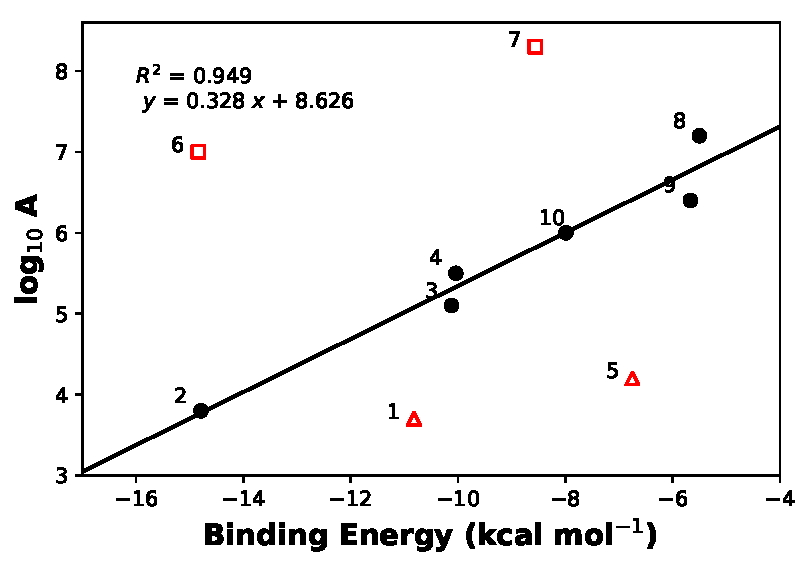
\includegraphics[width=0.75\textwidth]{figures/arrhenius-scatter.pdf}
  \caption[bleh]{bleh}
\label{fig:Arrhenius}
\end{figure}
